\documentclass[11pt]{article}
%% Package imports
\usepackage[utf8]{inputenc}
\usepackage{amsmath}
\usepackage{subcaption}
\usepackage{amsfonts}
\usepackage{amssymb}
\usepackage{physics}
\usepackage{graphicx}
\usepackage[left=1cm,right=1cm,top=2cm,bottom=2cm]{geometry}
\usepackage{multirow}
\usepackage{booktabs}
\usepackage{float}
\usepackage{verbatim}
\usepackage{amsthm}
\usepackage{minted}
\usepackage{fancyhdr}
\usepackage[dvipsnames]{xcolor}
\usepackage{parskip}
\usepackage{blindtext}
\usepackage{hyperref}
\usepackage{listings,xcolor}
\usepackage[T1]{fontenc}
\usepackage{xcolor}
\usepackage[scaled=0.9]{DejaVuSansMono}
\definecolor{commentgreen}{RGB}{2,112,10}
\definecolor{eminence}{RGB}{108,48,130}
\definecolor{weborange}{RGB}{255,165,0}
\definecolor{frenchplum}{RGB}{129,20,83}

\lstdefinelanguage{elixir}{
    morekeywords={case,catch,def,do,else,false,%
        use,alias,receive,timeout,defmacro,defp,%
        for,if,import,defmodule,defprotocol,%
        nil,defmacrop,defoverridable,defimpl,%
        super,fn,raise,true,try,end,with,%
        unless},
    otherkeywords={<-,->, |>, \%\{, \}, \{, \, (, )},
    sensitive=true,
    morecomment=[l]{\#},
    morecomment=[n]{/*}{*/},
    morecomment=[s][\color{purple}]{:}{\ },
    morestring=[s][\color{orange}]"",
    commentstyle=\color{commentgreen},
    keywordstyle=\color{eminence},
    stringstyle=\color{red},
	basicstyle=\ttfamily,
	breaklines,
	showstringspaces=false,
	frame=tb
}

\lstset{numbers=left,xleftmargin=2em,frame=single,framexleftmargin=0em,numberstyle=\footnotesize\ttfamily}
\renewcommand{\baselinestretch}{1.5}

%% Commands for inserting big braces.
\newcommand\lb{\left\lbrace}
\newcommand\rb{\right\rbrace}

%% Math symbols
\usepackage[shortlabels]{enumitem}
\usepackage{titling}
\setlength{\droptitle}{-3cm}

%% Page style settings
\pagestyle{fancy}
\fancyfoot{}
\fancyhead[L]{\slshape{Multi-Paxos}}
\fancyhead[R]{\slshape{Szymon Kubica, CID: 01871147}}
\fancyfoot[C]{\thepage}
\begin{document}

\title{Distributed Algorithms 60009 \ Coursework - Multi-Paxos}
\date{\today}
\author{Szymon Kubica, CID: 01871147}
 {\let\newpage\relax\maketitle}

\section*{Architecture}
At the top level of the system the Multipaxos module spawns a collection of
Servers and Clients and the Monitor which keeps track of the state of the whole
system. Each Server has its own Database, Replica, Leader and Acceptor. The
initial binding of the modules is done by Multipaxos, each replica gets bound
to all leaders and each leader gets bound to all acceptors and replicas,
each client gets access to all replicas. I omitted the corresponding \texttt{:BIND}
messages.
\begin{figure}[H]
    \centering
    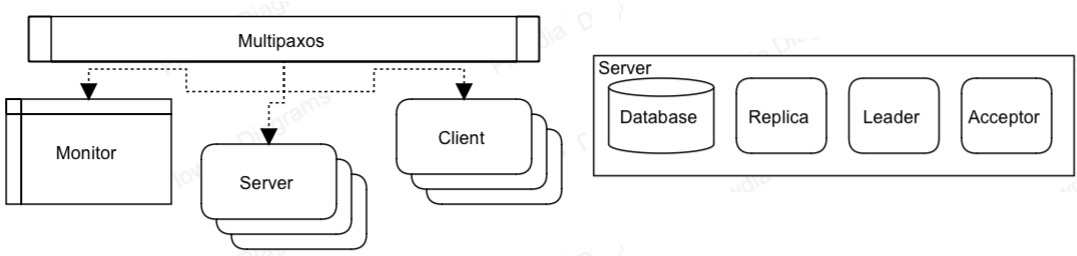
\includegraphics[width=400px]{architecture0.png}
    \caption{Top-level architecture.}
    \vspace{-15pt}
\end{figure}
A typical client request flow can be seen in Figure 2 below. The dotted arrows
represent spawned child processes, the black solid ones represent directed messages
with one recipient, whereas the blue ones represent messages which are broadcast
to all modules of a given type. Diagram on the left depicts the phase 1 of the synod protocol,
whereas phase 2 can be seen on the right. On the left one of the scouts
got preempted and one got adopted. On the right a commander got accepted
and broadcast its decision to all replicas which have
sent execute requests to the databases.
    \vspace{-5pt}
\begin{figure}[H]
    \centering
    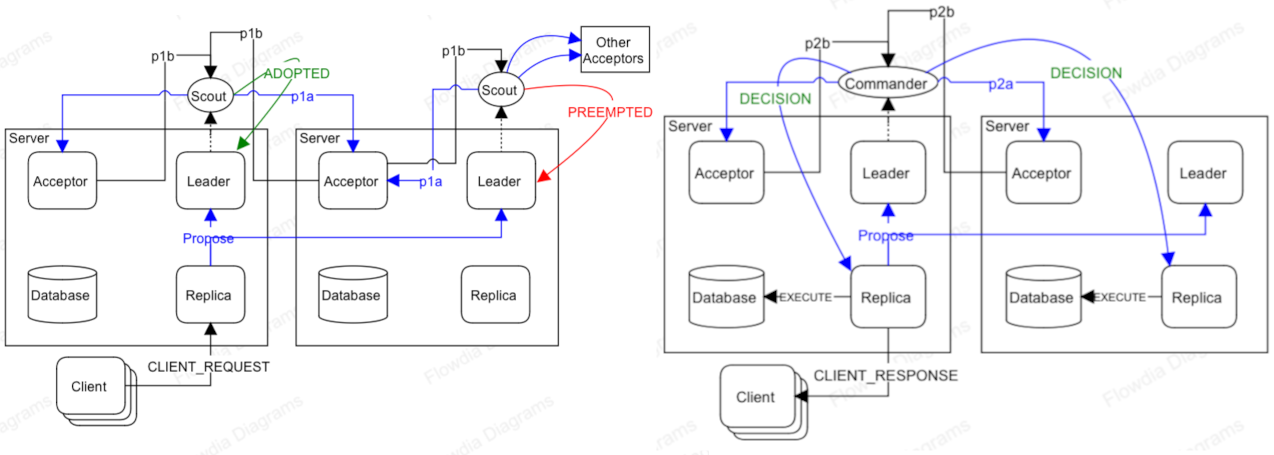
\includegraphics[width=\textwidth]{architecture1.png}
    \caption{Typical client request flow.}
\end{figure}

\pagebreak
\section*{Liveness}
My initial implementation of the section 3 followed closely the algorithm
described in the paper. Each leader after receiving a \texttt{:PREEMPTED}
message becomes inactive and starts pinging the leader that has preempted it,
instead of picking a higher ballot number and spawning a scout immediately. I
implemented that by spawning one failure detector module for each leader. When
preempted, a leader notifies its failure detector, which starts pinging the
leader associated with the preempting ballot \texttt{b}, then the leader
deactivates itself and continues .
\begin{lstlisting}[language=elixir, caption={New way of handling \texttt{:PREEMPTED} messages.},captionpos=b]
{:PREEMPTED, b} ->
  send(self.failure_detector, {:PING, b})
  self |> deactivate |> next
\end{lstlisting}
Each leader associates a timeout with its current ballot number. Every time a
leader gets preempted, its next ballot will use a longer timeout (multiplicative
increase). However, the timeout of the current ballot decreases linearly with each
proposal chosen for that ballot. It is done by sending an appropriate notification
from the commander after a \texttt{:DECISION} message is sent to the replicas.
Whenever an active leader gets pinged by FD of some other leader, it sends
its timeout back, and the FD updates it and uses it from now on.
\begin{lstlisting}[language=elixir, caption={Leader responding to a ping message.},captionpos=b]
{:RESPONSE_REQUESTED, requestor} ->
    cond do
      self.active -> send(requestor, {:STILL_ALIVE, ballot_num, timeout})
      self.preempted_by != nil -> send(requestor, {:STILL_ALIVE, preempted_by, timeout})
\end{lstlisting}
When tweaking the timeout settings, it was very difficult to pick the
appropriate constants. If the timeout decreased too quickly or it didn't grow
enough after preemptions, all leaders ended up preempting each other which
impacted performance. I noticed that we don't prioritise fairness, it is
perfectly fine if one leader is working on its ballot and all of the other ones
keep pinging it regularly and only react if they detect a failure. I added a
new version of the failure detector which has a static timeout. I realised that
it could happen that three leaders $\lambda_1$, $\lambda_2$,  $\lambda_3$
behave as follows: $\lambda_2$ preempts $\lambda_1$ and $\lambda_3$ preempts
$\lambda_2$, in which case $\lambda_2$ becomes inactive and stops responding to
$\lambda_1$'s pings, thus $\lambda_1$ wakes up and can possibly preempt
$\lambda_3$. Even though variable timeouts would help to solve this issue and
prevent it from live-locking, it introduces an unnecessary congestion. I solved
this problem by having each leader record the last preempting ballot number. If
a leader was recently preempted and is now inactive and gets pinged by somebody
whom he preempted before, it sends the ballot number that preempted it back to
the requestor (Listing2 above). That way the leader who pinged us doesn't wake up immediately
but starts pinging the leader who is currently working.
\pagebreak
\section*{Evaluation}
\subsection*{Hardware}
The evaluation was conducted on my laptop with the following specification:

OS: Linux 6.1.12-arch1-1, processor: 11th Gen Intel i7-1165G7 4.700GHz, cores: 8, ram: 32GB.

\begin{figure}[H]
    \centering
    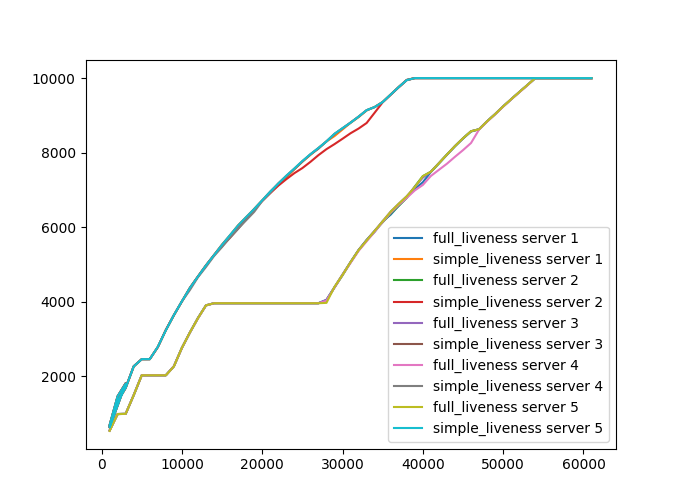
\includegraphics[width=400px]{full_liveness_vs_simple.png}
    \caption{Top-level architecture.}
    \vspace{-15pt}
\end{figure}

\begin{figure}[H]
    \centering
    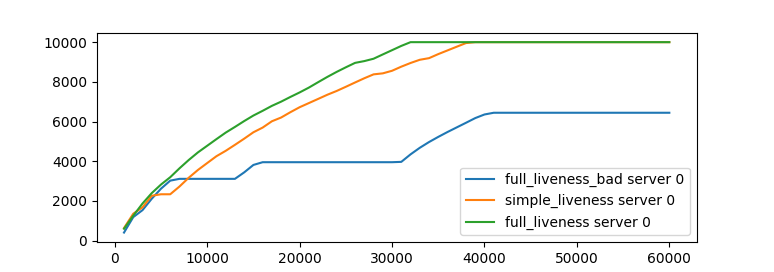
\includegraphics[width=400px]{liveness_simple_bad_config.png}
    \caption{Top-level architecture.}
    \vspace{-15pt}
\end{figure}

\subsection*{Live-locking Implementation and a Partial Fix}
\subsection*{Full Liveness and Simple Liveness}
\subsection*{Crash Failure of the Main Leader}
\end{document}
